\chapter{Resultados}

En este capítulo se presentan los datos obtenidos de la ejecución del proyecto bajo ciertas condiciones representativas, con la intención de validar la funcionalidad y también de encontrar los alcances y límites del mismo para el caso de clasificación planteado. Primero se estudia el tiempo de respuesta de los algoritmos de manera individual, a continuación el rendimiento en la configuración más simple, luego el sistema completo bajo condiciones varias, y por último se analiza la mejora introducida por el uso de la cache. Para la obtención de los datos que corresponden al sistema completo se utilizaron de manera complementaria scripts programados en lenguaje Python y en Bash. Durante todo el capítulo se usa LLU como acrónimo de \textit{Linear Look Up} y UTL para referirse al \textit{Unibit Trie Lookup}. 


\section{Stress de software}

Con la intención de obtener un gráfico que represente el rendimiento de los dos algoritmos implementados, se mide el retardo de búsqueda en función de la posición de coincidencia en la tabla de enrutamiento. Las pruebas se realizan de manera independiente a la Interfaz de acceso a la cabecera con el fin de aislar los efectos de la misma. En el eje de las abscisas se expresa la ubicación del prefijo más largo en una tabla de 100 elementos  y en las ordenadas se puede observar el tiempo de búsqueda en ciclos de reloj.

\begin{figure}[h]
  \centering
	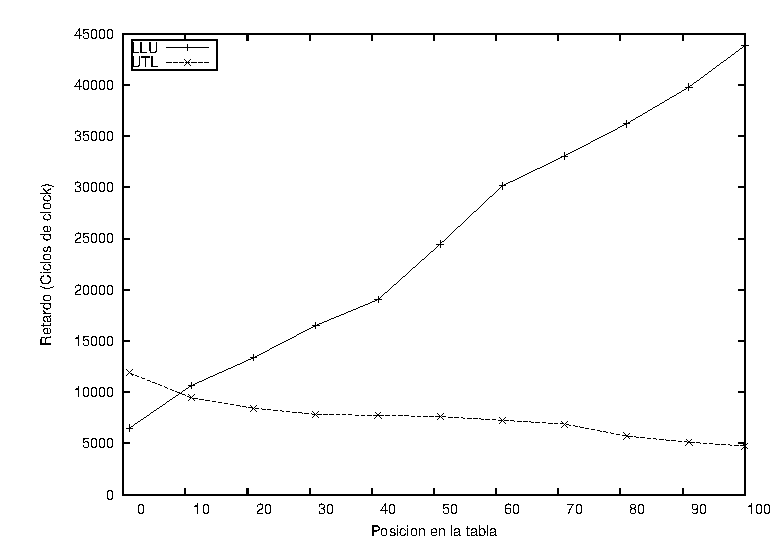
\includegraphics[width=0.8\textwidth]{5-resultados/graf/llu-utlsof.eps}
  \caption{Retardo de Búsqueda LLU vs UTL}
  \label{fig}
\end{figure}

Puede observarse que para LLU el tiempo es proporcional a la posición del prefijo dentro de la tabla. La misma se encuentra representada en una lista y por ello es necesario recorrerla hasta encontrar la coincidencia correspondiente. La cantidad de iteraciones depende del nodo en el cual se encuentre el prefijo. Para direcciones que se correspondan con la ruta por defecto se obtiene el mayor retardo, ya que la misma está almacenada en el último nodo.

En el caso de UTL los bits que conforman el prefijo se almacenan en un árbol binario. La cantidad de iteraciones depende entonces de la longitud del prefijo. Para este caso en particular el mayor de ellos tiene una longitud de 24 bits, por lo tanto se requieren 24 iteraciones como máximo, sea cual fuere el tamaño de la tabla de ruteo. La ruta por defecto (prefijo de longitud cero) tiene el menor retardo de búsqueda, ya que la misma está representada en el nodo raíz del árbol.

De todo esto surge la conclusión inmediata de que el tiempo medio de lookup tiene menos variabilidad en el caso UTL que en LLU. Si para este último se incrementa la cantidad de elementos en la tabla, dicho tiempo se verá incrementado también. Sin embtargo no se encontrarán variaciones en el tiempo medio para UTL ya que, como se mencionó anteriormente, este retardo depende de la longitud del prefijo y no del tamaño de la tabla.

\newpage
\section{Stress de hardware}
\begin{figure}[h]
  \centering
	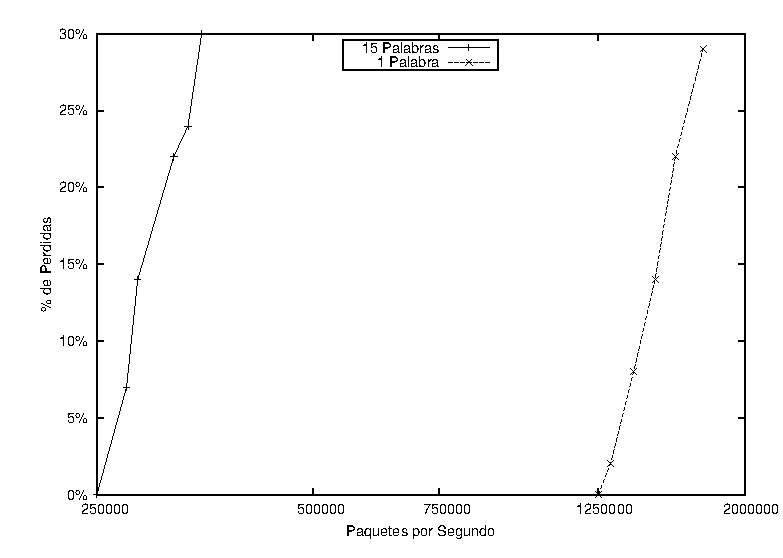
\includegraphics[width=0.70\textwidth]{5-resultados/graf/loop.eps}
  \caption{Caso Loopback para 1 y 15 palabras}
  \label{fig:loop}
\end{figure}
Se estudia en primer término el caso loopback a los fines de encontrar los límites superiores del sistema determinado por la sección hardware. En este caso el software solo se limita a recibir los datos e inmediatamente después confirma el procesamiento, enviando un resultado predefinido de regreso al hardware. Este test permite determinar la tasa mínima de pérdida introducida por la transferencia del paquete al microprocesador, sin aplicar algoritmo alguno de procesamiento en software. Esta pérdida se debe esencialmente a las latencias de transferencia a memoria y de transferencia por el bus Avalon. Se realizan las pruebas correspondientes para las dos versiones de Uplink.
En el eje de las abscisas de la figura \ref{fig:loop} es posible ver la cantidad de paquetes por segundo que se ingresan a la arquitectura. Los puntos que se encuentran sobre el eje corresponden entonces al caso de procesamiento de datos sin pérdida. En las ordenadas se puede observar la cantidad de paquetes perdidos en valores porcentuales. Para obtener esta métrica se procesó una cantidad constante de paquetes, 9000, y luego se contrastó este valor con un contador global que el generador coloca en la ultima palabra de cada paquete. Así se calculó la cantidad paquetes perdidos, sobre la cantidad total de paquetes generados. Este mismo sistema es el usado en todos los gráficos posteriores.


\newpage
\section{Implementación Completa}

En este ensayo se verifica el rendimiento del sistema implementado de manera completa. Se consideran tres situaciones que caracterizan los tiempos de procesamiento de los algoritmos: un punto mínimo que corresponde al menor tiempo de clasificación, un punto promedio que ejercita 10 entradas equidistantes a lo largo de la tabla y un punto máximo que indica el peor tiempo de clasificación posible para un algoritmo dado. 

\subsubsection{a) Linear Lookup (LLU)}
Se evalúa el desempeño para los casos en que se envían 1 y 15 palabras de 32 bits como ya se mencionó. Se observa que los valores de pérdida de paquetes para ambos casos difieren mucho para profundidades de búsqueda pequeña (figura \ref{figminllu}), pero convergen a medida que la profundidad de búsqueda aumenta (figuras \ref{figpromllu} y \ref{figmaxllu}). Este efecto era esperable ya que para accesos muy lentos a la tabla el retardo introducido por la transferencia de datos desde el  el hardware se vuelve despreciable.

\begin{figure}[!h]
  \centering
	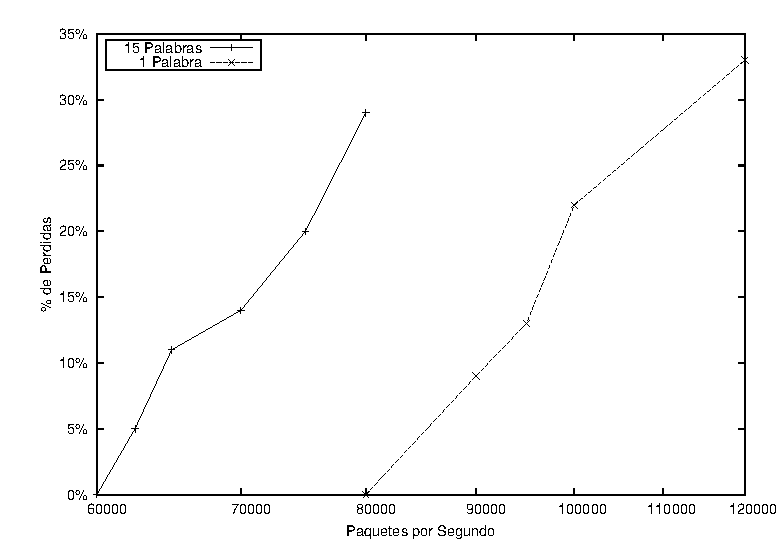
\includegraphics[width=0.7\textwidth]{5-resultados/graf/llumin.eps}
  \caption{Retardo mínimo LLU}
  \label{figminllu}
\end{figure}
\begin{figure}[!h]
  \centering
	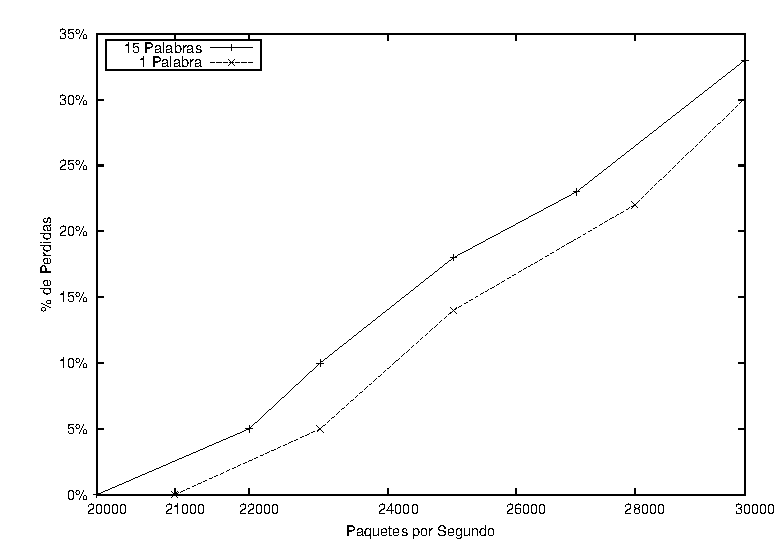
\includegraphics[width=0.7\textwidth]{5-resultados/graf/lluprom.eps}
  \caption{Retardo promedio LLU}
  \label{figpromllu}
\newpage
\end{figure}
\begin{figure}[!h]
  \centering
	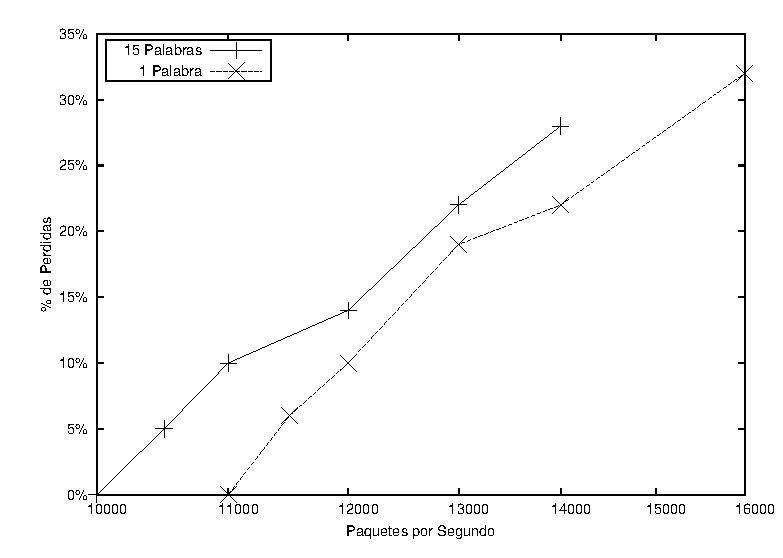
\includegraphics[width=0.7\textwidth]{5-resultados/graf/llumax.eps}
  \caption{Retardo máximo LLU}
  \label{figmaxllu}
\end{figure}



\newpage
\subsubsection{b) Unibit Trie Lookup (UTL) }

En los gráficos que corresponden al Unibit Trie Lookup es posible observar que existe una menor diferencia entre la máxima cantidad de paquetes que pueden ser transmitidos sin pérdida en cada una de las 3 situaciones. Por ejemplo, si se considera pérdida nula para la versión de Uplink que envía 15 palabras de 72 bits, se tiene una cantidad de 80000 paquetes para retardo mínimo, 65000 para retardo promedio y 50000 para el máximo retardo para UTL, contra 60000, 20000 y 10000 respectivamente para LLU. También la diferencia entre enviar el paquete entero y solo la IP destino se reduce, lo que da la pauta de que cuando el tiempo de acceso es uniforme el impacto de enviar 1 o 15 palabras tiende a ser menor.
%\newpage
\begin{figure}[!h]
  \centering
	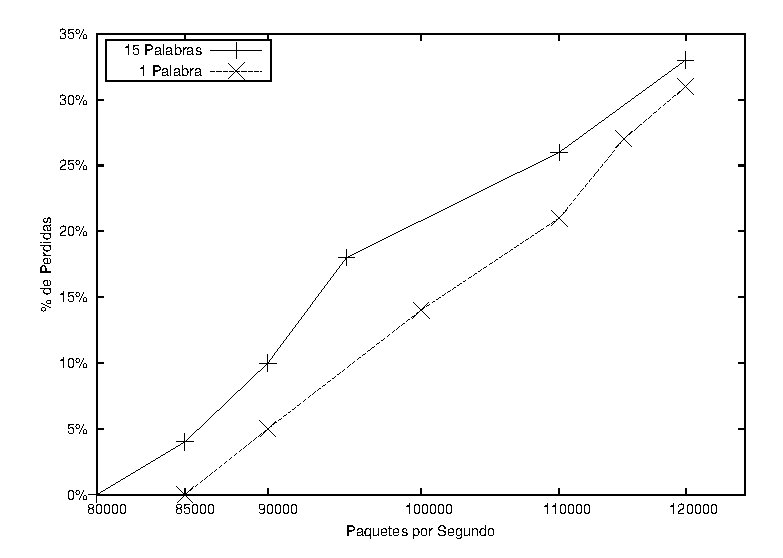
\includegraphics[width=0.7\textwidth]{5-resultados/graf/utlmin.eps}
  \caption{Retardo mínimo UTL}
  \label{fig}
\end{figure}
\begin{figure}[!h]
  \centering
	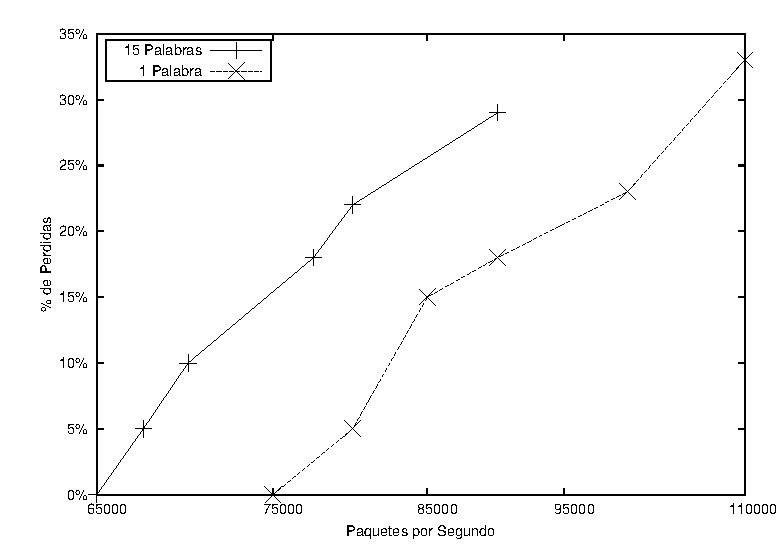
\includegraphics[width=0.7\textwidth]{5-resultados/graf/utlprom.eps}
  \caption{Retardo promedio UTL}
  \label{fig}
\end{figure}
\begin{figure}[!h]
  \centering
	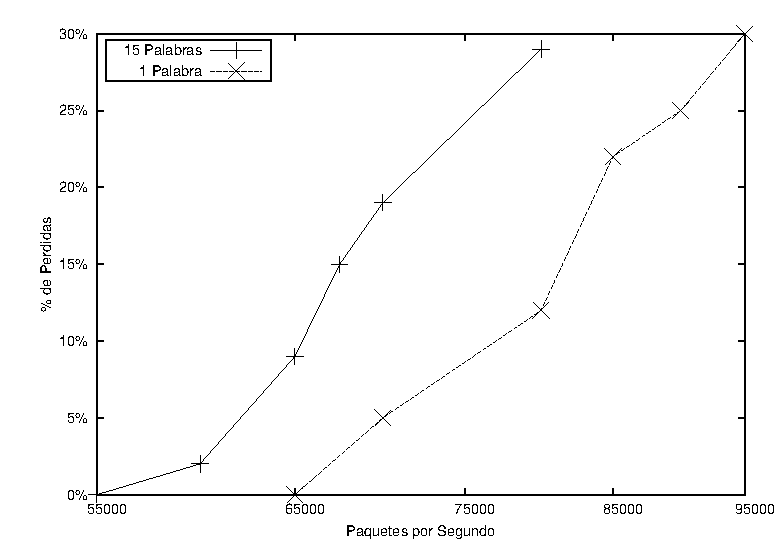
\includegraphics[width=0.7\textwidth]{5-resultados/graf/utlmax.eps}
  \caption{Retardo máximo UTL}
  \label{fig}
\end{figure}

\newpage
\subsubsection{Comparativa Inter-Algoritmos}
Se presenta a modo de comparación un gráfico que contiene el mínimo, el máximo y el promedio para la versión de Uplink que envía una sola una palabra con los dos algoritmos implementados. 
\begin{figure}[!h]
  \centering
	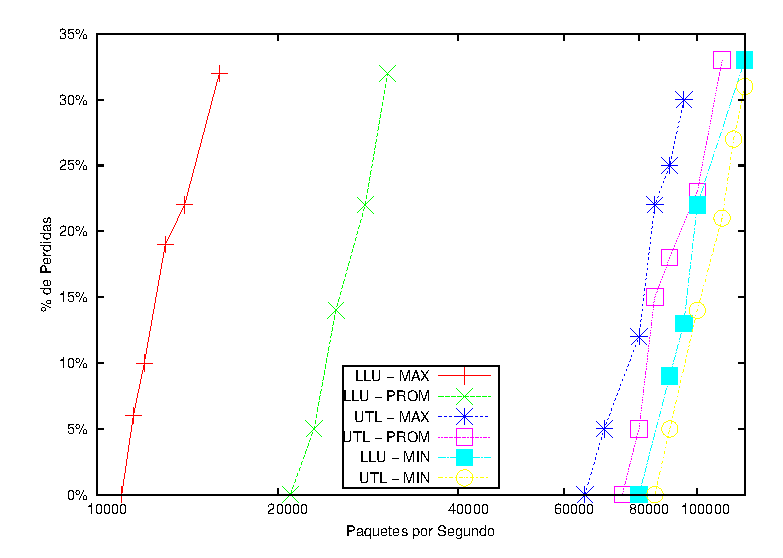
\includegraphics[width=0.7\textwidth]{5-resultados/graf/lluvsutl.eps}
  \caption{Comparativa UTL - LLU}
  \label{figvs}
\end{figure}

En la figura \ref{figvs} pueden apreciarse de una manera más global las diferencias en transmisión de paquetes sin pérdida. Como puede observarse, dichas diferencias se ven más acentuadas para los casos de LLU, debido a que este tipo de búsqueda es, como se mencionó anteriormente, altamente dependiente de la posición del prefijo dentro de la tabla de ruteo. No sucede esto con UTL ya que en este caso el tiempo de búsqueda está ligado a la longitud del prefijo y no a su posición dentro de la tabla.


\section{Caché}

La cache desarrollada para este proyecto está pensada a los fines de satisfacer la posibilidad de que varios paquetes consecutivos tengan una dirección IP destino que pertenezcan a un grupo común de flujos (flow locality). Con la implementación utilizada se logró un tiempo de acceso uniforme de alrededor de 1000 ciclos, tiempo varias veces menor que el mejor caso tanto en LLU (6400) como en UTL (5000). En la figura ~\ref{fig:cachecomp} se puede ver cómo el peor caso del algoritmo LLU soporta hasta 10000 paquetes por segundo sin cache, mientras que es capaz de procesar hasta 700000 paquetes por segundo con el agregado de la cache. Aunque este ejemplo sólo analiza el caso en el que son todos hits, es posible ver la mejora sustancial que implica el uso de una memoria de este tipo. 

\begin{figure}[!h]
  \centering
	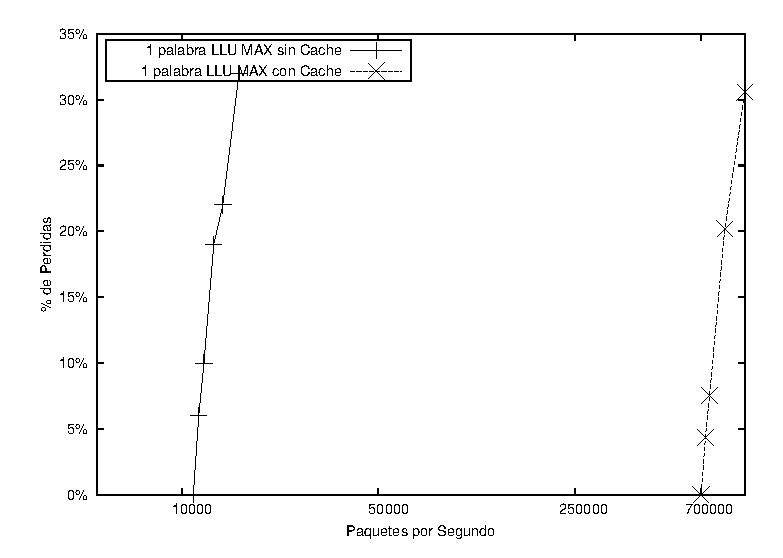
\includegraphics[width=0.7\textwidth]{5-resultados/graf/cachecomp.eps}
  \caption{Cache }
  \label{fig:cachecomp}
\end{figure}

